
%(BEGIN_QUESTION)
% Copyright 2006, Tony R. Kuphaldt, released under the Creative Commons Attribution License (v 1.0)
% This means you may do almost anything with this work of mine, so long as you give me proper credit

A simple form of electronic pressure transmitter could be made with a bourdon tube and a {\it Linear Variable Differential Transformer}, or {\it LVDT}:

$$\includegraphics[width=15.5cm]{i00183x01.eps}$$

Explain how this instrument works, what type of electrical output signal it generates (e.g. current, voltage, resistance, etc.), and what polarity (if any) that output signal has.

\underbar{file i00183}
%(END_QUESTION)





%(BEGIN_ANSWER)

Note very carefully how the two secondary coils are connected in series-opposing (as denoted by the phase dots)!  This detail is essential in figuring out how the LVDT works.

\vskip 10pt

The output is an AC voltage, the magnitude of which is proportional to core position, which in turn is proportional to applied pressure.  For what it's worth, the phase of the output voltage will be inverted with respect to the excitation voltage as the bourdon tube draws the core up:

$$\includegraphics[width=15.5cm]{i00183x02.eps}$$

LVDTs have several advantages over potentiometers:

\begin{itemize}
\item{} No friction
\item{} No wear
\item{} No potential to generate a spark in normal operating conditions
\end{itemize}

Their major disadvantage is requiring an AC excitation voltage.  The frequency of this excitation voltage is important as well: it must be much larger than the highest frequency of pressure changes you wish to measure (as per the Nyquist sampling theorem).

%(END_ANSWER)





%(BEGIN_NOTES)

%INDEX% Measurement, pressure: LVDT as bourdon tube sensor

%(END_NOTES)


